%%%%%%%%%%%%%%%%%%%%%%%%%%%%%%%%%%%%%%%%%%%%%%%%%%%%%%%%%%%%%%%%%%%%%%%%%%%%%%%%
%2345678901234567890123456789012345678901234567890123456789012345678901234567890
%        1         2         3         4         5         6         7         8

\documentclass[letterpaper, 10 pt, conference]{ieeeconf}  % Comment this line out if you need a4paper

%\documentclass[a4paper, 10pt, conference]{ieeeconf}      % Use this line for a4 paper

\IEEEoverridecommandlockouts                              % This command is only needed if
                                                          % you want to use the \thanks command

\overrideIEEEmargins                                      % Needed to meet printer requirements.

% See the \addtolength command later in the file to balance the column lengths
% on the last page of the document

% The following packages can be found on http:\\www.ctan.org
\usepackage{graphics} % for pdf, bitmapped graphics files
\usepackage{epsfig} % for postscript graphics files
%\usepackage{mathptmx} % assumes new font selection scheme installed
%\usepackage{times} % assumes new font selection scheme installed
\usepackage{amsmath} % assumes amsmath package installed
\usepackage{amssymb}  % assumes amsmath package installed
\usepackage{url}
\usepackage{subfigure}
% Rafael
\usepackage{xspace}
\usepackage{pgfplots}
\usepackage{graphicx}
\usepackage{epstopdf}
\usepackage{cite}
\usepackage{bm}


% axded by Rafael
%%%%%%%%%%%%%%%%%%%%%%%%%%%%%%%%%%%%%%%%%%%%%%%%%%%%%%%%%%%%%%%
\def\marhes{{\sc Marhes}\xspace}
\def\octor{{OctoRoACH}\xspace}
\def\octors{{OctoRoACHes}\xspace}
\def\turtle{{TurtleBot}\xspace}
\def\turtles{{TurtleBots}\xspace}
\newcommand{\ie}{{\it i.e.},\xspace}
\newcommand{\eg}{{\it e.g.},\xspace}
\newcommand{\cf}{{\it c.f.},\xspace}
\newcommand{\el}{{\it et al.},\xspace}
\newcommand{\etc}{\text{etc.}}

\providecommand{\norm}[1]{\left\lVert#1\right\rVert}

%% Math defs
% The set of reals, integers, etc.
\renewcommand{\Re}{\mathbb{R}}
\newcommand{\Ze}{\mathbb {Z}}
\newcommand{\Pe}{\mathbb {P}}
\newcommand{\I}{\mathcal{I}}

\newtheorem{definition}{Definition}
%%%%%%%%%%%%%%%%%%%%%%%%%%%%%%%%%%%%%%%%%%%%%%%%%%%%%%%%%%%%%%

\title{\LARGE \bf
Homework 3: Hidden Markov Models
}

\author{Luis A. Valbuena Reyes% <-this % stops a speeeeace
%\thanks{*This work was not supported by the MAST project.}% <-this % stops a space
\thanks{Luis Valbuena is with the Department of Electrical and Computer Engineering,
        University of New Mexico, Albuquerque, NM, 87131-0001, {\tt\small \{lavalbuenar@unm.edu\}}}%
}

\begin{document}

\newtheorem{theoremMyThesis}{Theorem}
\newtheorem{corollary}{Corollary}
\newtheorem{problemStatement}{Problem Statement}

\maketitle
\thispagestyle{empty}
\pagestyle{empty}


%%%%%%%%%%%%%%%%%%%%%%%%%%%%%%%%%%%%%%%%%%%%%%%%%%%%%%%%%%%%%%%%%%%%%%%%%%%%%%%%
\begin{abstract}

In this document, we present the solution for homework 3. Trying to follow the guidelines for writing papers, we develop each the requirements of the assignment on Sections \ref{sec:Theory}, \ref{sec:Experiments}, and \ref{sec:Conclusion}.
\end{abstract}

%%%%%%%%%%%%%%%%%%%%%%%%%%%%%%%%%%%%%%%%%%%%%%%%%%%%%%%%%%%%%%%%%%%%%%%%%%%%%%%%


\section{INTRODUCTION}
\label{sec:Intro}

In this document, we extend the Expectation Maximization approach to consider time, into what is known as hidden Markov models (HMM). Speech recognition is one
of some applications in which a group sounds are collected and the goal is to find out the words that were spoken. The sounds are perceived and the words related
to those sounds are the hidden variables\footnote{The words are hidden inside the sounds} and because the structure of language, we know of relationships among 
words: there are some words that come after others and in contrast, there are words that don't have any relation among them. This embeds the Markovian property 
into the problem, that is, given a sequence of transitions among states (words) $Z_{1}, Z_{2},\hdots,Z_{n},Z_{n+1}, \hdots$, we have that
\begin{equation*}
 \mathbb{P}(Z_{n+1} |Z_{n},\hdots, Z_{2},Z_{1}) =  \mathbb{P}(Z_{n+1} |Z_{n}),
\end{equation*} 
which means that the next state $Z_{n+1}$ on the sequence only depend on the current state $Z_{n}$ and it is not required to keep track of all the states prior to $Z_{n}$. The
transitions occur at equally spaced periods of time so we are studying a discrete Markov chain.

In our case, we are studying a signal that is corrupted with additive noise and we plan to model it with a HMM. We characterize a HMM with the following parameters (taken 
from\cite{HMM_Rabiner} ):

\begin{itemize}
\item $M$ The number of states. The states are hidden but we can assume a particular number of them.
\item $\mathbf{P}$ Transition probability matrix. The position $P_{ij}$ relates the probabilty of a transition from state $Z(i)_{n}$ to state $Z(j)_{n+1}$. The sumation of the element in each of  the
rows of $P$ are equal to $1$.
\item $\mathbf{\pi}$ The initial distribution.
\end{itemize}

We will denote the states as $Z(i)_{n}$ for $i \in \{ 1,2,\hdots,M\}$. The observation measured is $X_{n}$ where the subscript indicates the time $n$. Even though the states  $Z(i)_{n}$
have the Markovian property, the observations are independent among them, that is
\begin{equation*}
 \mathbb{P}(X_{n+1} |Z(j)_{n+1}Z(i)_{n}) =  \mathbb{P}(X_{n+1} |Z(j)_{n}),
\end{equation*} 
that is, the observation $X_{n+1}$ only depends of state $Z(\ast)_{n+1}$.

Although we are assuming a particular number of states $M$, we need to now the parameters $\mu_{i}$ and $\Sigma_{i}$ for the state $Z(i)$ as well as matrix $\mathbf{P}$ and the distribution  $\mathbf{\pi}$. In the next section, we present how to find these values.

%%%%%%%%%%%%%%%%%%%%%%%%%%%%%%%%%%%%%%%%%%%%%%%%%%%%%%%%%%%%%%%%%%%%%%%%%%%%%%%%


\section{Theory}
\label{sec:Theory}

Based on the material found in \cite{HMM_Rabiner} and \cite{bookML_Murphy}. Because of the iterative nature of the procedure behind HMM's, we can conveniently translate the problem posed at the end of 
Section \ref{sec:Intro} into the following three problems

\begin{itemize}
\item Given some sequence of observed values $\mathbf{X}_{i} = X_{1},X_{2},\hdots,X_{n},X_{n+1},...X_{T}$ and some preliminary values for $\mathbf{\pi}$, $\mathbf{P}$, $\mu_{i}$ and $\Sigma_{i}$ for $Z(i)_{n}$.
What is the probability of our HMM model to generate that sequence $\mathbf{X}_{i}$? See Sections \ref{sec:TheoryForwardsStep}, and \ref{sec:TheoryBackwardsStep}, and  \ref{sec:TheoryForwardsBackwardsStep}.
\item Given some sequence of observed values $\mathbf{X}_{i} = X_{1},X_{2},\hdots,X_{n},X_{n+1},...X_{T}$ and some preliminary values for $\mathbf{\pi}$, $\mathbf{P}$, $\mu_{i}$ and $\Sigma_{i}$ for $Z(i)_{n}$. How do we choose a sequence of states $\mathbf{Z}_{i} = Z(\ast)_{1},Z(\ast)_{2},\hdots,Z(\ast)_{n},Z(\ast)_{n+1},...$ that has the best measure of reproducing  $\mathbf{X}_{i}$? See Sections \ref{sec:TheoryForwardsBackwardsStep} and \ref{sec:TheoryViterbiAlgorithm}.
\item How can we modify $\mathbf{\pi}$, $\mathbf{P}$, $\mu_{i}$ and $\Sigma_{i}$ for $Z(i)_{n}$ so we maximize the values calculated in the two previous questions? See Section \ref{sec:TheoryBaumWelchAlgorithm}.
\end{itemize}

In the following Sections we explain the idea behind each Step as well as the mathematical expressions used Section \ref{sec:Experiments}

\subsection{Forwards Step}
\label{sec:TheoryForwardsStep}

The  calculation $\mathbb{P}(\mathbf{X}_{i})$ given some previous model parameters would be

\begin{equation}
    \mathbb{P}(\mathbf{X}_{i}) = \sum_{\text{all } \mathbf{Z}} \mathbb{P}(\mathbf{X}_{i}|\mathbf{Z}) \mathbb{P}(\mathbf{Z})
    \label{eq:TooOperations}
\end{equation}
where all the possible sequences $\mathbf{Z}$ are the same length as $\mathbf{X}_{i}$. However, the number of operations involved is overwhelming. An optimal 
calculation consists of looking at a local perspective by considering a particular state $Z(i)_{n}$ at time $n$ and looking forward and backwards in time for recursion 
expressions. When looking forward in time, we want to calculate the probability of all the possible states in time $n-1$ that can visit $Z(i)_{n}$ on the next transition.
We regard the forwards step recursively as
 
\begin{equation*}
    \bm{\alpha}_{n} \varpropto \bm{\psi}_{n} ( \mathbf{P}^T \odot \bm{\alpha}_{n-1}),
\end{equation*}
where $ \psi(i)_{n} = \mathcal{N}(X_{n}|\mu_{i},\Sigma_{i})$ and $\odot$ is the Hadamard product. Each $ \bm{\alpha}_{n}$ needs to be normalized and  $ \bm{\alpha}(i)_{1} = \frac{1}{M}$.

\subsection{Backwards Step}
\label{sec:TheoryBackwardsStep}

Following the previous discussion, we also need to go backwards in time and we do that by calculating  the probability of all the possible states in time $n+1$ that can be visited
from $Z(i)_{n}$ on the next transition. That is the backwards term and is expressed as 

\begin{equation*}
    \bm{\beta}_{n} = \mathbf{P} ( \bm{\psi}_{n+1} \odot \bm{\beta}_{n+1}).
\end{equation*}

Note that $\bm{\beta}_{n}$ need not be normalized. However, the initial condition is $\bm{\beta}(i)_{T} = 1$.


\subsection{Forwards-Backwards Step}
\label{sec:TheoryForwardsBackwardsStep}

The optimal equivalent to Equation \ref{eq:TooOperations} is given by the Forwards-Backwards step as

\begin{equation*}
    \bm{\gamma}_{n} \varpropto ( \bm{\alpha}_{n} \odot \bm{\beta}_{n}),
\end{equation*}
where $\bm{\gamma}_{n}$ in normalized.

Evolution of parameters $\bm{\alpha}_{n}$, $\bm{\beta}_{n}$ , and $ \bm{\gamma}_{n}$ can be seen on Fig.~\ref{fig:Alpha}, Fig.~\ref{fig:Beta}, and
Fig.~\ref{fig:Gamma}.

\subsection{The Baum-Welch Algorithm}
\label{sec:TheoryBaumWelchAlgorithm}

The Baum-Welch Algorithm is the Expectation Maximization for HMM.  First, we need to compute matrix $\bm{\xi}_{n,n+1}$ as 

\begin{equation*}
    \bm{\xi}_{n,n+1} \varpropto P \odot (\bm{\alpha}_{n}(\bm{\psi}_{n+1} \odot \bm{\beta}_{n+1})^{T}).
\end{equation*}

Then, the Expectation step involves the following calculations

\begin{equation*}
\begin{aligned}
     \mathbb{E}[N_{k}^{1}] &= \sum_{i=1}^{M} \gamma_{i,1}(k),\\
     \mathbb{E}[N_{j}] &= \sum_{i=1}^{M}  \sum_{n=1}^{T} \gamma_{i,n}(j),  \\
     \mathbb{E}[N_{ik}] &= \sum_{i=1}^{M}  \sum_{n=1}^{T} \xi_{i,n}(j,k),
\end{aligned}
\end{equation*}
where the notation changes slightly: the subindex $i$ refers to a realization $\mathbf{X}_{i}$ and the original notation $\xi_{n,n+1}$ changes to $\xi_{i,n}$ to make
reference to $\mathbf{X}_{i}$.

In the Maximization step we compute

\begin{equation*}
\begin{aligned}
     P_{j,k} &= \frac{\mathbb{E}[N_{ik}]}{\sum_{k^{\prime}} \mathbb{E}[N_{i k^{\prime}}]},\\
     \bm{\pi} &= \frac{ \mathbb{E}[N_{k}^{1}]}{N},  \\
     \mu_{k}&= \frac{ \sum_{i=1}^{M}  \sum_{n=1}^{T} \gamma_{i,n}(k)X_{i,n}}{ \mathbb{E}[N_{k}]}, \\
     \Sigma_{k} & = \frac{ \sum_{i=1}^{M}  \sum_{n=1}^{T} \gamma_{i,n}(k)X_{i,n}X_{i,n}^T - \mu_{k}\mu_{k}^{T}}{\mathbb{E}[N_{k}]}
\end{aligned}
\end{equation*}
where $N$ is the number of realizations.

It is suggested in \cite{bookML_Murphy} for the initialization stage to neglect time and execute an Expectation Maximization with Gaussian Mixture Models or K-means
on the observed data and then use these values to start  the Baum-Welch algorithm.

\subsection{The Viterbi Algorithm}
\label{sec:TheoryViterbiAlgorithm}

The Viterbi Algorithm is a recursive expression intended to establish a sequence on states  $\mathbf{Z}_{i}$ given a sequence of observations $\mathbf{X}_{i}$. The
recursive expression is given by

\begin{equation*}
   \delta_{n}(j) = \max_{i}{ \{ \delta_{n-1}(i) \mathbf{P}_{ij}  \psi(i)_{n} \}},
\end{equation*}
with the initial condition
\begin{equation*}
   \delta_{1}(j) =   \pi_{j}  \psi_{1} .
\end{equation*}

Another criteria to determine the best  $\mathbf{Z}_{i}$ is using $\gamma$, i.e., $Z_{n}^{\ast} =  \max_{i}{  \{ \gamma(i)_{n} \}} $.
%%%%%%%%%%%%%%%%%%%%%%%%%%%%%%%%%%%%%%%%%%%%%%%%%%%%%%%%%%%%%%%%%%%%%%%%%%%%%%%%


\section{Experiments}
\label{sec:Experiments}

We can think of the artificially generated data as an arriving signal which contains noise. The signal has three states i.e., $\mu_{1} = 1$, $\mu_{2} = 2$, 
and $\mu_{3} = 3$ and the standard deviation of the noise is $\sigma = 0.3$. The observed variable is the signal with the noise. The data is generated 
using the script given in the assignment. The transition probability matrix of the Markov chain is:

\begin{equation*}
 P = \begin{bmatrix}
            0.8 & 0.1 & 0.1 \\
            0.2 & 0.5 & 0.3 \\
            0.3 & 0.1 & 0.6 
        \end{bmatrix}.
\end{equation*}  

A preliminary estimation on matrix $P$ is done by counting the transitions on the generated signal, the result is given by 
\begin{equation*}
 P_{est1} = \begin{bmatrix}
           0.7895 & 0.1066 & 0.1039\\
           0.2085 & 0.4583 & 0.3331\\
           0.3119 & 0.1047 & 0.5834
        \end{bmatrix}.
\end{equation*}  

A realization of the observed variable and the state is presented on Fig.~\ref{fig:ObservedvariableX} and Fig.~\ref{fig:ObservedvariableZ}.
\begin{figure}[ht!]
 \begin{center}
  	\subfigure[\label{fig:ObservedvariableX}]{\includegraphics[width=0.48\textwidth,trim=5 15 5 8]{Drawings2/ObservedvariableX.eps}}
 	\subfigure[\label{fig:ObservedvariableZ}]{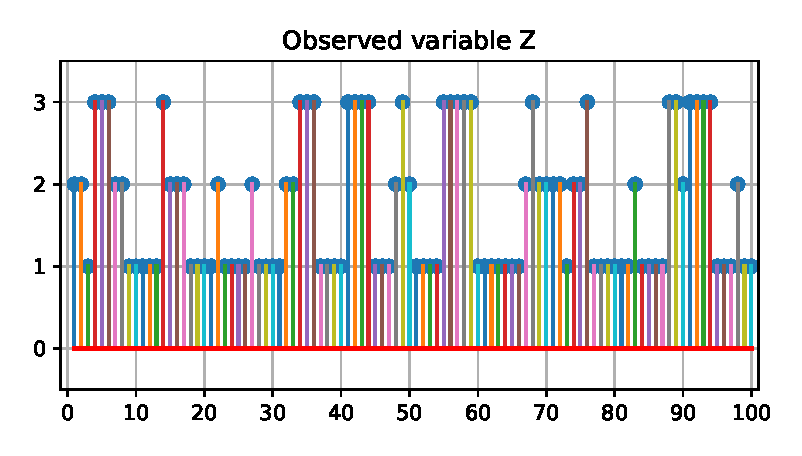
\includegraphics[width=0.48\textwidth,trim=5 15 5 8]{Drawings2/ObservedvariableZ.eps}}
         \caption{A realization of the artificially generated data  (a) Observed variable, (b) Real state. }
 \end{center}
\end{figure}

In the execution of our experiments we conducted $80$ realizations. For the realization of Fig.~\ref{fig:ObservedvariableX} and Fig.~\ref{fig:ObservedvariableZ}, the evolution of the forwards term are depicted in Fig.~\ref{fig:Alpha(1)}, Fig.~\ref{fig:Alpha(2)}, and Fig.~\ref{fig:Alpha(3)}; while the backwards term is presented in Fig.~\ref{fig:Beta(1)}, Fig.~\ref{fig:Beta(2)}, and Fig.~\ref{fig:Beta(3)}. Finally graphs for the forwards-backwards terms is depicted in Fig.~\ref{fig:Gamma(1)}, Fig.~\ref{fig:Gamma(2)}, and Fig.~\ref{fig:Gamma(3)}.

Consider the region $60 \leq n \leq 66$ on the horizontal axis of all the figures. Note on Fig.~\ref{fig:ObservedvariableZ} that the signal stays on the state $1$ for that period and   Fig.~\ref{fig:Alpha(1)} and Fig.~\ref{fig:Gamma(1)} coincide to point their maximum over that region too.

Now consider  the region $15 \leq n \leq 18$, where the state is $2$. Now Fig.~\ref{fig:Alpha(1)} and Fig.~\ref{fig:Gamma(1)} show that region to be minimal while Fig.~\ref{fig:Alpha(2)} and Fig.~\ref{fig:Gamma(2)} coincide to point their maximum over that region. A similar reasoning for state $3$ can be drawn on the region  $55 \leq n \leq 59$.

Unfortunately, these characteristics are not clearly present on the backwards term displayed  on  Fig.~\ref{fig:Beta}.  This suggest a serious implementation problem that cascades through the Baum-Welch algorithm. 
The final results for the transition probability matrix and the stationary distribution are given by

\begin{figure}[ht!]
 \begin{center}
  	\subfigure[\label{fig:Alpha(1)}]{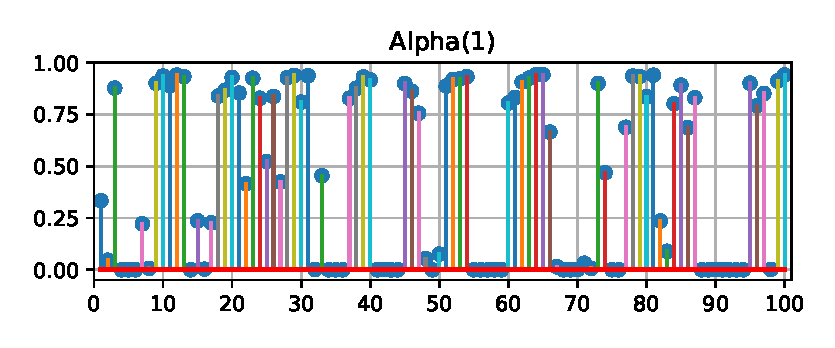
\includegraphics[width=0.5\textwidth,trim=5 15 5 1]{Drawings2/Alpha(1).eps}}
 	\subfigure[\label{fig:Alpha(2)}]{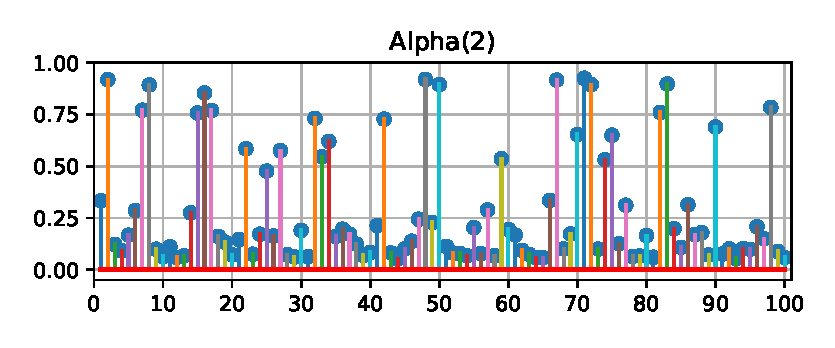
\includegraphics[width=0.5\textwidth,trim=5 5 5 1]{Drawings2/Alpha(2).eps}}
 	\subfigure[\label{fig:Alpha(3)}]{\includegraphics[width=0.5\textwidth,trim=5 5 5 1]{Drawings2/Alpha(3).eps}}
         \caption{Forwards term for  states (a) $1$, (b) $2$, (c) $3$. }
 \label{fig:Alpha}
 \end{center}
\end{figure}
 
\begin{figure}[ht!]
 \begin{center}
  	\subfigure[\label{fig:Beta(1)}]{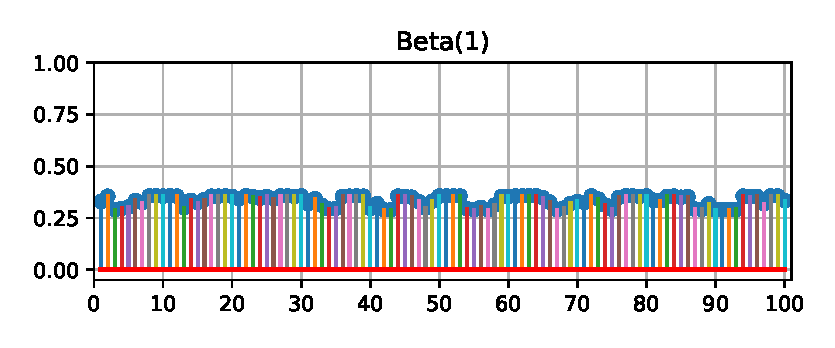
\includegraphics[width=0.5\textwidth,trim=5 15 5 1]{Drawings2/Beta(1).eps}}
 	\subfigure[\label{fig:Beta(2)}]{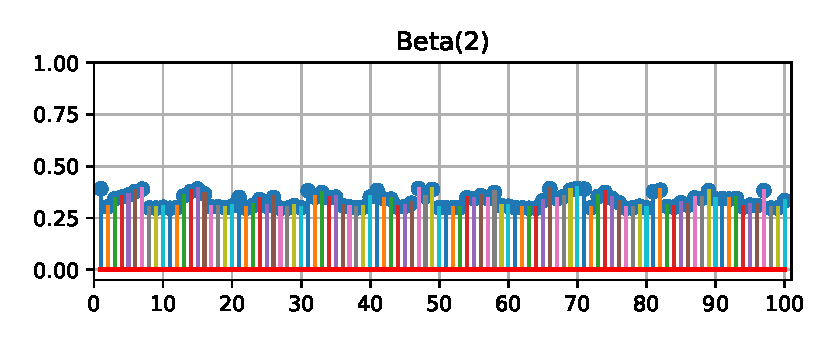
\includegraphics[width=0.5\textwidth,trim=5 5 5 1]{Drawings2/Beta(2).eps}}
 	\subfigure[\label{fig:Beta(3)}]{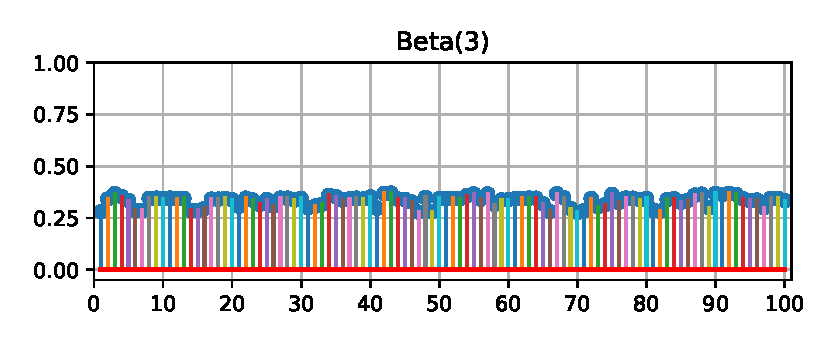
\includegraphics[width=0.5\textwidth,trim=5 5 5 1]{Drawings2/Beta(3).eps}}
         \caption{Backwards term for states (a) $1$, (b) $2$, (c) $3$. }
 \label{fig:Beta}
 \end{center}
\end{figure} 

\begin{figure}[ht!]
 \begin{center}
  	\subfigure[\label{fig:Gamma(1)}]{\includegraphics[width=0.5\textwidth,trim=5 15 5 1]{Drawings2/Gamma(1).eps}}
 	\subfigure[\label{fig:Gamma(2)}]{\includegraphics[width=0.5\textwidth,trim=5 5 5 1]{Drawings2/Gamma(2).eps}}
 	\subfigure[\label{fig:Gamma(3)}]{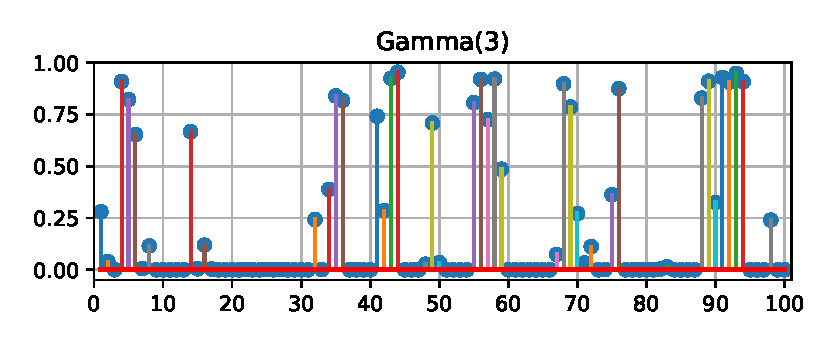
\includegraphics[width=0.5\textwidth,trim=5 5 5 1]{Drawings2/Gamma(3).eps}}
         \caption{Forwards-Backwards for states (a) $1$, (b) $2$, (c) $3$. }
 \label{fig:Gamma}
 \end{center}
\end{figure}

\begin{equation*}
 P_{HMM} = \begin{bmatrix}
          0.5104 & 0.2878 & 0.2017\\
          0.4146 & 0.3479 & 0.2374\\
          0.4983 & 0.2369 & 0.2647
        \end{bmatrix},
\end{equation*}  

\begin{equation*}
 \bm{\pi}_{HMM} = \begin{bmatrix} 0.5247\\ 0.2497\\ 0.2256\end{bmatrix}.
\end{equation*}  

Even though a fixed number of iterations were commanded without relying on the calculation of the log-likelihood, it might be possible
that we are not letting the algorithm run for long enough. However, by inspecting Fig.~\ref{fig:EvolutionParameters} we can see that means 
and sigmas converge within the preestablished number of iterations.

\begin{figure}[ht!]
 \begin{center}
  	\subfigure[\label{fig:EvolutionMeans}]{\includegraphics[width=0.5\textwidth,trim=5 15 5 1]{Drawings2/EvolutionMeans.eps}}
 	\subfigure[\label{fig:EvolutionSigmas}]{\includegraphics[width=0.5\textwidth,trim=5 5 5 1]{Drawings2/EvolutionSigmas.eps}}
         \caption{Forwards-Backwards for states (a) $1$, (b) $2$. }
 \label{fig:EvolutionParameters}
 \end{center}
\end{figure}

%%%%%%%%%%%%%%%%%%%%%%%%%%%%%%%%%%%%%%%%%%%%%%%%%%%%%%%%%%%%%%%%%%%%%%%%%%%%%%%%

\section{Conclusion}
\label{sec:Conclusion}

We have presented the methodology employ to study HMM on a academic example of a corrupted signal. We presented the theory behind the modeling 
of such phenomenon using HMM's. We attempted to support our claims with simulation results approximating the parameters of the artificially generated
data. However,  Fig.~\ref{fig:Beta} suggest that the backwards expression is not correctly implemented.  As a consequence, the estimation done on the
maximization step are corrupted.

We implemented the forwards, backwards and forwards-backwards steps using both index notation as well as matrix format with no improvement.

There were suspicions about not letting the algorithm execute enough iterations but the convergence shown in Fig.~\ref{fig:EvolutionParameters} indicates 
otherwise.
 


%%%%%%%%%%%%%%%%%%%%%%%%%%%%%%%%%%%%%%%%%%%%%%%%%%%%%%%%%%%%%%%%%%%%%%%%%%%%%%%%

%References are important to the reader; therefore, each citation must be complete and correct. If at all possible, references should be commonly available publications.


%\pagebreak

\bibliographystyle{IEEEtran}
\bibliography{References}

%%%%%% APPENDIX %%%%%%%
%q\input{Appendix}
\end{document}
